
\documentclass[xcolor=x11names,compress]{beamer}


\usetheme[num]{SmartSerif}

\usepackage{graphicx}
\DeclareGraphicsExtensions{.pdf,.png,.jpg}
\graphicspath{{./images/}}
\usepackage{color}

\usepackage{subcaption}



% ---------------------------------------------------------------------------------------
% Thanks to http://www.guidodiepen.nl/2009/07/creating-latex-beamer-handouts-with-notes/
 % \usepackage{handoutWithNotes}
 % \pgfpagesuselayout{4 on 1 with notes}[a4paper,border shrink=5mm]
 % \pgfpagesuselayout{2 on 1 with notes landscape}[a4paper,border shrink=5mm]
% ---------------------------------------------------------------------------------------

\setcounter{tocdepth}{2}

\title{Using Life-Logging to Re-Imagine Representativeness in Corpus Design}
\author{Stephen Wattam}
\institute[2013]{Lancaster University}
\date{\tiny \today}

\begin{document}

\maketitle

\frame{\frametitle{Contents}
    \tableofcontents
}




% -----------------------------------------------------------------------------------------
% \frame{\frametitle{Balance/Representativeness}
% 
%         % Representativeness is, simply:
%         Maximising the extent to which a sample resembles the population
% 
%         % For a given question 
%         % For a given population (needs defining)
% 
% 
%         \begin{itemize}
%             \item \textbf{Balance/Proportionality}---The ability of each sample to relate to its real-world counterpart
%                 % As seen in some given dimension
%                     
%             \item \textbf{Size}---The ability to adequately represent sub-populations fully for subsampling and specific inquiry
%                 % i.e. is there enough data on a given subtype of language?
%         \end{itemize}
% 
%         Language is so complex that, to satisfy these for a given research question, we require a very large sampe size
% 
% \note{}
% }
% 

\section{Sampling Design}



\subsection{Conventional Sampling}
\frame{\frametitle{Conventional Corpus Design}
    \begin{itemize} 
        \item Samples texts as instances of a persistent construct
            \vspace{10pt}
    % i.e. books themselves, rather than the act of reading

\item Stratified along genre, medium, etc.
            \vspace{10pt}
    % This differs from social science samples, who usually use variation across
    % the social population
    % 
    % There's a fair amount of disagreement on what variables are most important still
    %
    % It's not possible to sample consumption/production without having better information on these

\item Based on available indexes such as bestseller lists
            \vspace{10pt}
    % i.e. bestseller lists, etc

\item Tightly coupled to expert opinion on text importance
    % Which lists to use, etc, is chosen by committee
    % these have direct influence on content (selecting more books, for example)

\end{itemize}

\note{
    BNC: "Texts were chosen for inclusion according to three selection features: domain (subject field), time (within certain dates) and medium (book, periodical, etc.)."
}
}


\frame{\frametitle{Difficulties}
    \begin{itemize}
        \item Many variables don't have indexes
            \vspace{10pt}
            % (i.e. production vs consumption)
        \item Ethical or legal concerns limit some types of data
            \vspace{10pt}
            % i.e. speech vs writing proportions
        \item Selection using `proxy variables', due to lack of auxiliary data
            \vspace{10pt}
            % and these have interactions with other variables of interest, i.e. p[in index list] correlates with some social/linguistic property
        \item True empirical distribution of many variables is unknown
            % leading to unrepresentative choices for stratum size
            % such as time authored/read vs "was made in this year"
    \end{itemize}

    \note{}
}



% TODO: the slide below 
% \subsection{Literature}
% \frame{\frametitle{Literature}
%     \begin{itemize}
%         \item Biber
%         \item Varadi
%         \item Leech
%         \item
%     \end{itemize}
% \note{}
% }

% NOTE: another approach here would be to send out questionnaires in order to assess
%       the social validity of corpus results, i.e. to check the indexes.

\subsection{Demographic Sampling}
\frame{\frametitle{Demographic Sampling}
    \begin{itemize}
    
        \item Views language use as a social event
            \vspace{10pt}
% a language transaction, a la Leech

\item Stratified along demographic variables
            \vspace{10pt}
% as in the BNC's demographic speech sample
% as with virtually all other social science samples

\item Expert opinion only needed to select demographics
            \vspace{10pt}
% though sample size is still a hot topic and always will be
% population is now "all users of x language",
% the users can be determined through other surveys

\item Opportunities for census of language genres
% Constant recording can record everything, for once
% Personal corpus stuff.

\end{itemize}
    % \begin{itemize}
    %     \item 

    %     \item Selecting different variables of interest re-orients many practical issues
    %     % back to basics --- what is the aim of CL?
    %     \item I've chosen to sample language as a social, transitive, event
    %         % i.e. for a given group of people, what language do they use?
    %     \item Sample proportions of language use 'in the wild'
    %     \item With sufficient sample size, this is equivalent, however, pragmatic sampling issues differ greatly
    % \end{itemize}
\note{}
}


\frame{\frametitle{Advantages}
    \begin{itemize}
        \item Social demographics are well documented
            \vspace{10pt}
        \item No central index is required 
            \vspace{10pt}
            % The person is a central index
        \item Additional variables are exposed to study
            \vspace{10pt}
            % production/consumption, time/context etc.
            % more variables, i.e. not only author/title/genre (which may still be there),
            % but also social ones and transitive ones
        \item Discovery of language types/uses possible
            % ephemera, TV, labels, billboards etc

    \end{itemize}

\note{}
}


\frame{\frametitle{New Difficulties}
    \begin{itemize}
        \item Sampling text from many people is technically demanding, expensive
            \vspace{10pt}
            % We have to leave the office more
            % technology makes this easier nowadays
            % This is also an issue for things like the BHPS
        \item Size issues now affect `how many people'
            \vspace{10pt}
            % difficult even for simple data
            % dependent on the variability of people's everyday usage (a la biber)
        \item Multi-modal sources require transcription 
            % but this can be helped by using the sample as auxiliary data
            % Many things don't start of so well curated
    \end{itemize}
\note{}
}




\section{Life-Logging}
\subsection*{History}
\frame{\frametitle{Life-Logging}
    \begin{itemize}
        \item Continual verbatim recording/broadcasting of life
        \item Originally for entertainment (JenniCam, Justin.tv)
        \item Heavily reliant on portable technology, connectivity

            \vspace{10pt}
\begin{figure}
        \centering
        \begin{subfigure}[b]{0.5\textwidth}
                \centering
                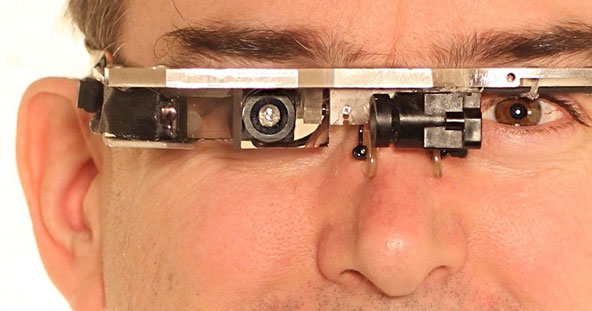
\includegraphics[width=\textwidth]{mann}
        \end{subfigure}%
        ~ %add desired spacing between images, e. g. ~, \quad, \qquad etc.
          %(or a blank line to force the subfigure onto a new line)
        \begin{subfigure}[b]{0.35\textwidth}
                \centering
                
\includegraphics[width=\textwidth]{jennicam}
        \end{subfigure}
\end{figure}

    \end{itemize}
\note{}
}


\subsection*{Application to Corpus Design}
\frame{\frametitle{Applications}
    \begin{itemize}
        \item Memory augmentation: Steve Mann, SenseCam, Machine Listening
            \vspace{10pt}
        \item Information retrieval: DARPA LifeLog
            \vspace{10pt}
        \item Language acquisition: Deb Roy
            \vspace{10pt}
        \item Corpus Building: LLC, BNC (sort of)
            \vspace{10pt}
        \item Posterity/Narcissism: Dymaxion Chronofile, JenniCam
    \end{itemize}
\note{
    BNC: "Recruits who agreed to take part in the project were asked to record all of their conversations over a two to seven day period."
    BNC: "Given that we were not attempting to represent the complete range of age and social groups within each region..."
}
}



\section{Method}
\frame{\frametitle{}

    \begin{center}
    \sc \Large Preliminary Study 
    \end{center}

    % TODO: slide needs some work
\note{}
}

\subsection*{Aims/RQs}
\frame{\frametitle{Aims}
Construct a personal corpus, to determine:

    \begin{itemize}
        \item What proportions of language types I use
        \item If any types of language are missing entirely from existing corpora
            % Yes, Chomsky was correct ;-)
        \item Relative proportions of text and speech
        \item Practical methods for deployment using other subjects
        \item Time required to build a useful sample size
            %(based on variation seen, temporal cyclic stuff);
    \end{itemize}

% In addition to this, I have a number of studies planned using the data, but those can wait
\note{}
}

\frame{\frametitle{Process}
    \begin{itemize}
        \item Record all language used (produced or received), in all formats.
            \vspace{10pt}
        \item Compile daily lists of language types used
            \vspace{10pt}
        \item Transcribe and convert logs into a usable corpus.
            % What constitutes long enough?
    \end{itemize}
\note{}
}



\section{Data Collection}
\subsection*{Methods}
% What to record
% 'later lookup'/notes
% trade-off between seamlessness and comprehensiveness
\frame{\frametitle{Collection Strategy}
    \begin{itemize}
        \item Focus on unobtrusive, recall-based logging
            \vspace{10pt}

        \item Daily journal of language use:
            \begin{itemize}
                \item Listings of language used
                \item Subjective descriptions of which sections were read
                \item Details of complex interactions (shopping, music)
                \item Annotation of daily continuous logs
            \end{itemize}

    \end{itemize}
\note{}
}

% Methods (one slide each?)
%  - technical
%   - squid
%   - recording (a/v)
%   - blog
%   - notebook
\frame{\frametitle{Data Sources}

Persistent resources 
%may be retrieved easily and need not be recorded verbatim
    \begin{itemize}
        \item Books
            \vspace{10pt}
        \item Music
            \vspace{10pt}
        \item Audio/video, recorded
            \vspace{10pt}
        \item Handwritten notes
    \end{itemize}

\note{}
}

\frame{\frametitle{Data Sources 2}
 
Ephemeral resources
%must be recorded verbatim, or are impractical to recall
    \begin{itemize}
        \item Speech
            \vspace{10pt}
        \item Billboards; advertising; labelling
            \vspace{10pt}
        \item Broadcast media
            \vspace{10pt}
        \item Todo lists, personal notes
            \vspace{10pt}
        \item Talking to myself
    \end{itemize}



\note{}
}

\frame{\frametitle{Data Sources 3}

Resources of digital origin 
%are generally easier to capture verbatim

    \begin{itemize}
        \item Documents, presentations and other files
            \vspace{10pt}
        \item Website contents; emails
            \vspace{10pt}
        \item Web chat logs
            \vspace{10pt}
        \item CLI terminal usage; keyboard input
    \end{itemize}

\note{}
}


\frame{\frametitle{Journal}
The journal is formed from a physical notebook:

\begin{center}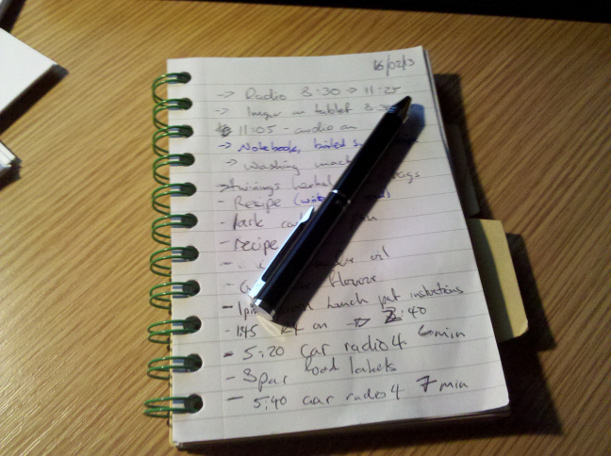
\includegraphics[width=3cm,height=2cm]{notebook}\end{center}

And an online log, which contains more detail:

    \begin{itemize}
        \item Music listened to
        \item Details of complex activities I'm likely to forget
            %(items bought at shops, etc)
        \item Subjective estimates of proportions read from various sources
            %(web pages, books, etc)
    \end{itemize}
\note{}
}


\frame{\frametitle{Audio Recording}

\begin{center}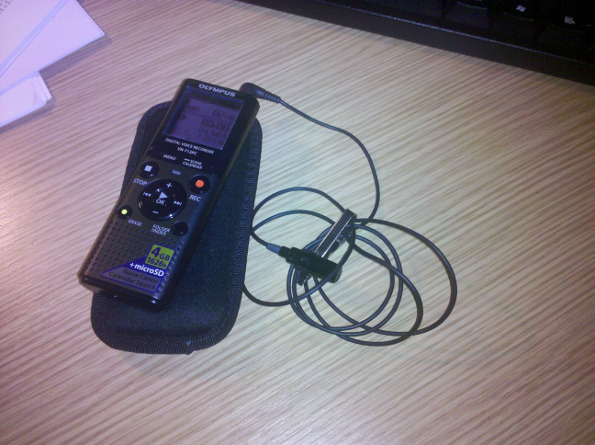
\includegraphics[width=4cm]{dictaphone}\end{center}
    
    \begin{itemize}
        \item Allows capture of small-scale speech events
        \item Difficult to process post-hoc without index markers, but realtime annotation is harder
        \item The law prevents external access without consent
    \end{itemize}

    \pause

 \begin{center}\alert{Ethical issues abound!}\end{center} 
\note{}
}


\frame{\frametitle{Video Recording}

\begin{center}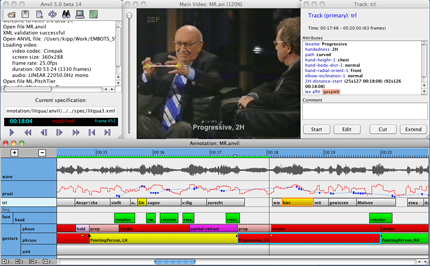
\includegraphics[width=4cm]{anvil5}\end{center}

    \begin{itemize}
        \item Detailed multi-media recording for awkward situations
        \item Useful when driving for road signs, music, GPS instructions, etc.
        \item Difficult to annotate without 100\% time overhead
    \end{itemize}
\note{}
}

 \frame{\frametitle{Technical---Web}
\begin{center}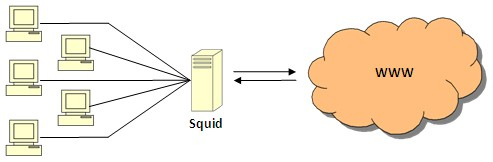
\includegraphics[width=7cm,height=2cm]{squid}\end{center}
    \begin{itemize}
        \item SQUID Proxy logs all traffic from my devices
        \item Heavy post-processing necessary:
            \begin{itemize}
                \item Removal of AJAX, automated, unread data
                \item Filtering of tags, boilerplate
                \item Removal of unread sections of text
            \end{itemize}
        \item A bot monitors web chat when I start speaking, and only logs when I am active
    \end{itemize}
\note{}
}

\frame{\frametitle{Technical---Other Digital Resources}
\begin{center}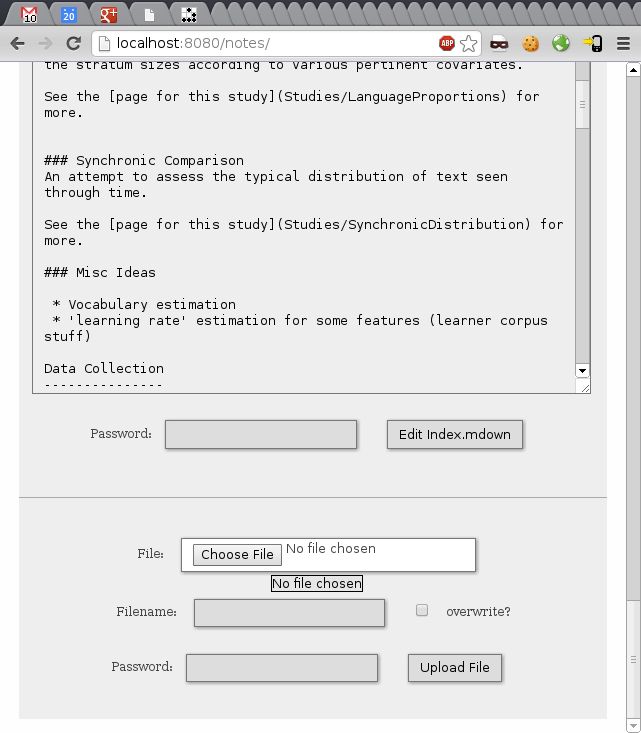
\includegraphics[width=3cm]{wik}\end{center}

    \begin{itemize}
        \item The journal and file store are accessible via the web
        \item Any files can simply be uploaded, or
        \item A flash drive can be used for large files
    \end{itemize}
\note{}
}


\frame{\frametitle{Technical---Input}
\begin{center}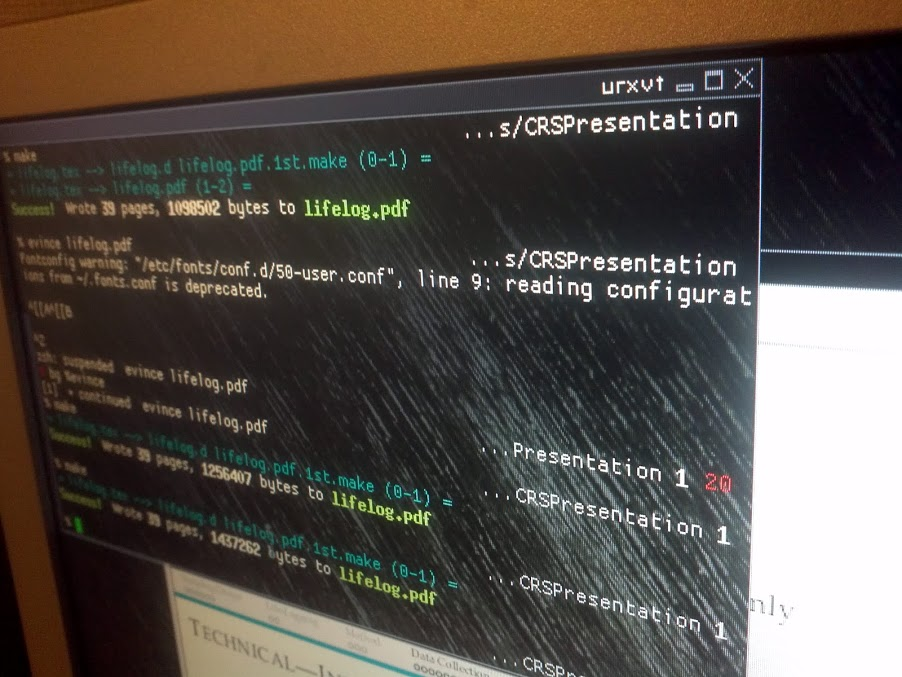
\includegraphics[width=4cm]{terminal}\end{center}
    \begin{itemize}
        \item Terminal-logging software can record all CLI use
        \item Keyloggers can capture all input, but often lack context information
        \item Email, web chat, other documents are all logged and timestamped anyway
    \end{itemize}
\note{}
}




\frame{\frametitle{Digitisation}

\begin{columns}[t]
    \column{.6\textwidth}

        \begin{itemize}
            \item Cameraphone for billboards and packages
            \vspace{5pt}
            \item Thanks to tumblr, no-one cares that I'm taking a photo of some cereal packets in public
            \vspace{5pt}
            \item Longer documents can usually be scanned
        \end{itemize}

    \column{.4\textwidth}
        \begin{center}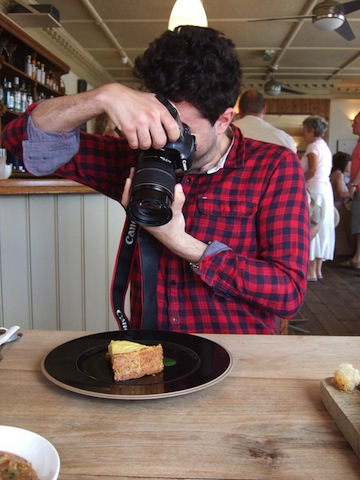
\includegraphics[width=4cm]{food-blogger}\end{center}
\end{columns}

\note{}
}




\subsection*{Transcription}
% How to convert and transcribe data from disparate sources
% information processing, organisation, markup
\frame{\frametitle{Operationalisation}
    \begin{itemize}
        \item Only `easily lost' data is transcribed during the study (daily)
            \vspace{5pt}
        \item Variable selection deliberately small to minimise interruptions
            \vspace{5pt}


        \item Audio, Video are most problematic
            \vspace{5pt}

        \item Data stored centrally for easy lookup

        % \item Digital documents require significant post-processing to remove unread content
        %     % markup, or simply bits I don't read of web pages
        %     % most terminal output is unread
        %     % I'm not *always* reading web chat
        % \item Audio needs to be annotated for genre, particpant count, etc. or transcribed
        % \item Pictures require transcription
        % \item Notebook metadata needs tabulating (and, in many cases, completing)
        % \item Web logs need downloading, post-processing
    \end{itemize}
\note{}
}


\section{Use} 
\subsection*{Use}
% Use as auxiliary data
% Resampling
% The idea of gathering more people's info
% Digital-only corpora for web scraping and rabalancing
% subject-specific corpora
\frame{\frametitle{Direct Use}
    \begin{itemize}
        \item NLP models for `custom' interaction with devices and services
            \vspace{5pt}
            % google's personal search, sat nav
        \item Balancing of corpora to specific demographics or people
            \vspace{5pt}
        \item Contextualisation of utterances with peer groups, etc
            \vspace{5pt}
        \item Comparison to existing language resources
            \vspace{5pt}
        \item Application to theories of lexical priming, language acquisition
    \end{itemize}
\note{}
}

\frame{\frametitle{Methods for auxiliary data}
    \begin{itemize}
        \item Conventional corpora may be resampled to build a larger corpus
            \vspace{10pt}
        \item Inspecting similar demographics from existing corpora indicates the differences in bias between both methods
        % TODO
    \end{itemize}
\note{}
}


\section{Findings \& Discussion}
\subsection*{Findings}
% Check prelim report
\frame{\frametitle{Findings --- Linguistic}
I read a very eclectic mix of things, including:
            % In one day, for example, I read articles on music theory, a guidebook for climbers, food cooking instructions, brand names on many items of clothing and food, instructions for how to do various things, GPS instructions and maps, and road signs.
            % This implies that a good representative sample will require a lot more text than first suspected
            % Low signal-noise ratio: That is, a corpus will have to grow rather large before it includes any whole books, let alone a cross-section of genres.

            \vspace{10pt}
\begin{columns}
    \column{.5\textwidth}
        \begin{itemize}
            \item Articles on music theory
            \item A recipe for boiled sweets
            \item A Map
            \item Many brand names
            % \item ~3 hours of radio 4
        \end{itemize}
    \column{.5\textwidth}
        \begin{itemize}
            \item p274 of 'Lancashire Rock'
            \item Inumerable road signs
            \item Cooking instructions
            \item Car GPS instructions
        \end{itemize}
\end{columns}

...and that's only written material.

\note{}
}

\frame{\frametitle{Findings --- Linguistic 2}
I rarely read \textsl{all} of \textsl{anything}, and often skip:
            % Correlates with design advice for the web, but I often read only one or two lines of comment
            \vspace{10pt}
\begin{itemize}
    \item Comments on web pages
            \vspace{10pt}
    \item Absolutely everything on many web pages
            \vspace{10pt}
    \item Almost all content in factual texts
\end{itemize}
\note{}
}

\frame{\frametitle{Findings --- Linguistic 3}
Text can sneak up on you
            % I find myself subconsciously absorbing text without really actively reading it. This covers things like TV subtitles and quick notes for myself, as well as things like advertising, calendars, branding, etc.
            % I have to train myself to notice language use

            \vspace{10pt}
\begin{figure}
        \centering
        \begin{subfigure}[b]{0.3\textwidth}
                \centering
                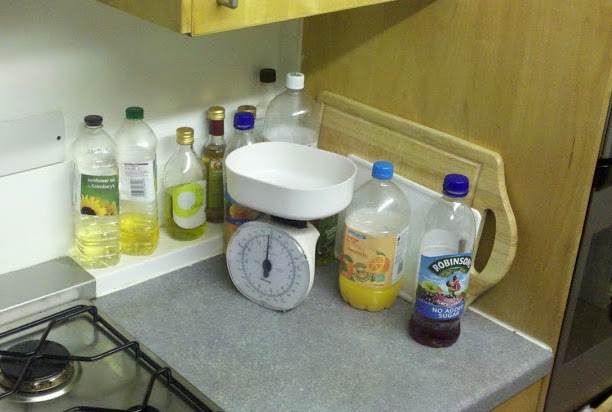
\includegraphics[width=\textwidth]{kitchen}
        \end{subfigure}%
        ~ %add desired spacing between images, e. g. ~, \quad, \qquad etc.
          %(or a blank line to force the subfigure onto a new line)
        \begin{subfigure}[b]{0.3\textwidth}
                \centering
                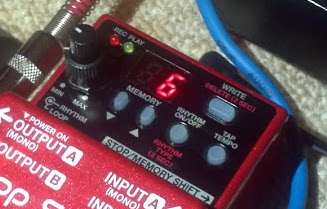
\includegraphics[width=\textwidth]{pedals}
        \end{subfigure}
        ~ %add desired spacing between images, e. g. ~, \quad, \qquad etc.
          %(or a blank line to force the subfigure onto a new line)
        \begin{subfigure}[b]{0.3\textwidth}
                \centering
                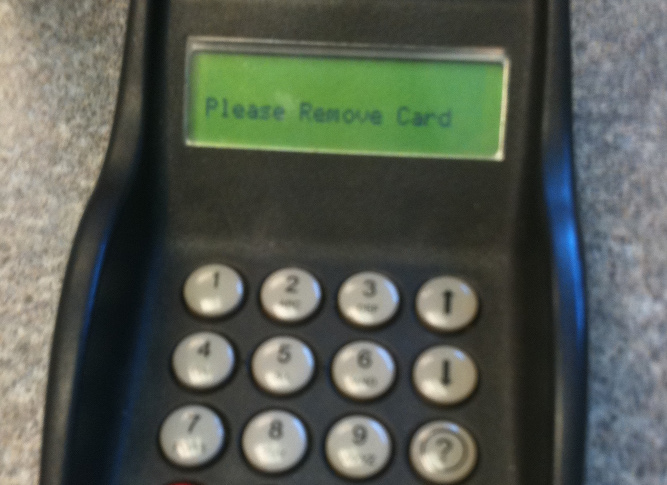
\includegraphics[width=\textwidth]{cpin}
        \end{subfigure}
\end{figure}

            \vspace{10pt}
            How many of these do I really \textsl{read} in everyday use?

\note{}
}

\frame{\frametitle{Findings --- Linguistic 4}
        I read a very large number of very small texts
            % contrary to most corpora
            \vspace{10pt}
\begin{itemize}
    \item Typically informative, and 1-2 sentences in length.  
            \vspace{10pt}

    \item Many would only read once or twice ever, such as parking machine instructions or button labels
\end{itemize}
\note{}
}

\frame{\frametitle{Findings --- Linguistic 5}
Due to radio/music, I often absorb more than one source of text at once

            \vspace{10pt}
\begin{itemize}
    \item Most smaller reading events were done whilst listening to radio 4
            \vspace{10pt}
    \item It's unclear how my attention divides itself
\end{itemize}
        
\note{}
}

\frame{\frametitle{Findings --- Linguistic 6}
    The vast majority of text I read is digital, but the vast majority of text sources I read are not.
            \vspace{10pt}
    \begin{itemize}
        \item Caused by my use of news websites, Wikipedia
            \vspace{10pt}
        \item Contrasts with my subjective preference for reading `real' books over ebooks
    \end{itemize}

\note{}
}



\frame{\frametitle{Findings --- Methodological}
Proper annotation requires a fair amount of neurolinguistic knowledge:
            \vspace{10pt}
    \begin{itemize}
        \item How often does one read a document when writing it?
        \item How deliberately must one read something for it to `count'?
        \item What's the best method of recording multiple parallel activities?
        \item What of programming languages, music, numeric and symbolic information, maps, etc.?
    \end{itemize}
\note{}
}


\subsection*{Ethics}
\frame{\frametitle{Ethics}
Covert research is always ethically suspect, however:

    \begin{itemize}
        \item Data being captured is not sensitive
        \item There is no other way to capture small spoken utterances
        \item Little to no human listening ever occurs on the resultant data
        \item Automated obfuscation is possible if only taking word counts/proportions
            % such as garbling the speech without affecting frequencies, allowing VAD to still work
        \item Data may be optionally deleted after (nightly) notation in the log 
            % unless sampling verbatim recordings, any data sampled may be deleted after its main points have been
            % noted down.
    \end{itemize}
\note{
  BNC: announced their recordings and allowed for deletion on request
}
}



\section*{Summary}
\frame{\frametitle{Summary}
    \begin{itemize}
        \item One preliminary test complete 
        \item Sampling methods need refinement, but show promise
        \item Annotation should be continuous in order to reduce bulk of transcription effort
        \item Though a single-person sample is useful, multiple people could augment data using questionnaires and data mining
        
        \vspace{10pt}
        \item I welcome questions/feedback on methods for the next round of sampling!
    \end{itemize}
\note{}
}


\appendix

% Which variables are collected
\frame{\frametitle{Collected Variables}
    Variables for capture in daily log: 
    \begin{itemize}
        \item Genre/Type (free coded)
        \item Age
        \item Author
        \item Title
        \item Setting
        \item Notes (i.e. times read, any notable properties of context and/or consumption)
    \end{itemize}
\note{}
}
\frame{\frametitle{Annotated Variables}
    Variables for annotation in final corpus
    \begin{itemize}
        \item Authorship
        \item Size of intended readership
        \item Text status (new, revised etc)
        \item Language
        \item Author gender
        \item Factuality
        \item Famliarity with intended readership
    \end{itemize}
\note{}
}

% -----------------------------------------------------------------------------------------
% 
% \frame{\frametitle{}
% \begin{columns} 
%     \begin{column}[c]{5cm} 
%     \end{column} 
%     \begin{column}[c]{5cm} 
%     \end{column} 
% \end{columns}
% 
% \note{}
% }
%
%
% \frame{\frametitle{}
%     \begin{itemize}
%         \item
%     \end{itemize}
% \note{}
% }
%
% \frame{\frametitle{}
% \note{}
% }
% -----------------------------------------------------------------------------------------
\end{document}
